\section{Körpererweiterungen; algebraische und transzendente Elemente}

\begin{df}\label{skript:13.1}
	Sei $L$ ein Körper und $K$ ein Teilkörper von L.
	Dann nennen wir $L$ eine \bi{Körpererweiterung} von $K$\index{Körper!Erweiterung}
	und schreiben $L \supseteq K$.
	In der Literatur wird auch oft $L | K $ geschrieben.
	Wir nennen 
	\begin{align*}
	| L : K | := \dim_K L
	\end{align*}
	den \bi{Grad} bzw. \bi{Körpergrad} von $L$ über $K$.\index{Körper!Grad}
\end{df}

\begin{genericdf}{Beispiele}\label{skript:13.2}\
	\begin{enumerate}
		\item[\textbf{(1)}]
		Für $\C \supseteq \R$ gilt $| \C : \R | = 2$.
		
		\item[\textbf{(2)}]
		Für $\R \supseteq \Q$ gilt $|\R : \Q| = \infty$.
		
		\item[\textbf{(3)}]
		Sei $f \in K[x]$ irreduzibel.
		Dann ist nach \ref{skript:9.10}
		\begin{align*}
		\underbrace{K[x] / (f) }_{:= L} \supseteq K
		\end{align*}
		eine Körpererweiterung mit $| L : K | = \Grad(f)$.
	\end{enumerate}
\end{genericdf}

\begin{genericdf}{Primkörper}\label{skript:13.3}
	Sei $L$ ein Körper,
	dann bezeichnen wir mit $\langle 1 \rangle$ den kleinsten Teilkörper von $L$,
	der die $1$ enthält.
	Wenn $\Char L = p$ ist, gilt $\langle 1 \rangle \cong \Z / p \Z$
	und wenn $\Char L = 0 $ ist, gilt $\langle 1 \rangle \cong  \Q$.
	Wir nennen $\Z / p \Z$ bzw. $\Q$ \bi{Primkörper}.\index{Körper!prim}
	Falls $|L | < \infty$ ist, so gilt $\Char L = p$.
	Damit folgt $| L : \Z / p \Z | < \infty$ und $|L | = p^m$.
\end{genericdf}

\begin{df}\label{skript:13.4}
	Sei $L \supseteq K$ eine Körpererweiterung und $\alpha \in L$.
	Nach \ref{skript:8.8} existiert ein Einsetzungshomomorphismus
	\begin{align*}
	\sigma_\alpha : K[x] \to L, f \mapsto f(\alpha).
	\end{align*}
	Wir setzen $K[\alpha] = \lbrace f(\alpha) \ | \ f \in K[x] \rbrace = \Bild \sigma_\alpha$.
	Da $K[x]$ ein Hauptidealring ist, gilt
	$\Ker \sigma_\alpha = 0$ oder $\Ker \sigma_\alpha = (\mu_\alpha)$ für ein $0 \neq \mu_\alpha \in K[x]$.
	Falls $\Ker \sigma_\alpha  = 0 $ ist, nennen wir $\alpha$ \bi{transzendent über $K$}.
	\index{transzendent}
	Sollte $\Ker \sigma_\alpha = ( \mu_\alpha) $ sein,
	nennen wir $\alpha$ \bi{algebraisch über $K$}.
	\index{algebraisch}
	Sind alle $\alpha \in L$ algebraisch über $K$, nennen wir $L \supseteq K$ \bi{algebraisch}
	Wenn $\mu_\alpha$ normiert ist, nennen wir $\mu_\alpha $ \bi{Minimalpolynom}.
\end{df}

\begin{generic_no_num}{Bemerkung}
	$K[\alpha]$ ist ein Körper, also ein Teilkörper von $L$.
\end{generic_no_num}

\begin{proof}
	Mit dem Homomorphiesatz folgt $K[\alpha] \cong K[x] / (\mu_\alpha)$.
	Damit ist $K[x] / (\mu_\alpha)$ ein Integritätsring und mit \ref{skript:9.2}
	ist $\mu_\alpha$ irreduzibel.
	Nun ist $K[x]$ ein Hauptidealbereich, also folgt mit \ref{skript:9.9}
	die Körpereigenschaft.
\end{proof}

\begin{genericdf}{Beispiele}\label{skript:13.5}\
	\begin{enumerate}
		\item[\textbf{(1)}]
		Für $\C \supseteq \R$ und $f=x^2+1$ gilt $f(i)=0$. $f$ ist das Minimalpolynom von $\i$, da irreduzibel und normiert.
		\item[\textbf{(2)}]
		Für $\R \supseteq \Q$, $f=x^4-2$ und $\alpha=\sqrt[4]{2}\in\R^+$ gilt $f(\alpha)=0$. $f$ ist das Minimalpolynom von $\alpha$, da irreduzibel (nach dem Eisenstein-Kriterium, $p=2$) und normiert.
		\item[\textbf{(3)}]
		Für $\C \supseteq \R$ und $\alpha=\i+\sqrt{2}$:
		\[\alpha^2=1+2\i\sqrt{2}, \ \alpha^3=5\i-\sqrt{2}, \ \alpha^4=-7+4\i\sqrt{2}=2\alpha^2-9.\]
		Das Polynom $f=x^4-2x^2+9$ ist normiert. $f$ ist irreduzibel, da: In $\Z/2\Z[x]$ ist $f=x^4+1$ irreduzibel (vgl. \ref{skript:10.5} \textbf{(3)}). $f(\alpha)=0$, also ist $f=\mu_\alpha$.
	\end{enumerate}
\end{genericdf}

\begin{genericdf}{Lemma}\label{skript:13.6}\
	Ist $|L:K| <\infty$, dann ist die Körpererweiterung $L\supseteq K$ algebraisch.
\end{genericdf}

\begin{proof}
	Sei $\alpha\in L$, $n=|L:K|$. Dann sind $1, \alpha, \alpha^2, \ldots, \alpha^n$ linear abhängig über $K$. Somit existieren $a_i\in K$, sodass
	\[a_0+a_1\alpha+\ldots+a_n\alpha^n=0\]
	und mindestens ein $a_i\neq0$. D. h. es gibt ein Polynom $f\in K[x]$, $f\neq0$ mit $f(\alpha)=0$, also ist $\Ker \sigma_\alpha\neq0$ und $\sigma_\alpha$ nicht injektiv. Also ist $\alpha$ algebraisch.
\end{proof}

\begin{genericdf}{Beispiel}\label{skript:13.7}\
	Sei $|L:K|=2$ und $\Char K\neq2$. Dann ist $L\supseteq K$ algebraisch und es existiert ein $\beta\in L$ mit $\beta^2\in K$ und $\beta\notin K$, denn:\\
	Es gibt ein $\alpha\in L$, sodass $\{1,\alpha\}$ eine $K$-Basis von $L$ ist. D. h. $L=K[\alpha]$ und
	\[\alpha^2=a\alpha+b\]
	mit $a,b\in K$. Da $\Char K\neq2$ ist, gibt es ein $c\in K$ mit $a=2c$. Also folgt
	\[\alpha^2=2c\alpha+b\]
	und daraus
	\[(\alpha-c)^2=b+c^2.\]
	Setzt man $\beta:=\alpha-c$, folgt: $\{1,\beta\}$ ist $K$-Basis von $L$, $L=K[\beta]$, $\beta^2\in K$, $\beta\notin K$.
\end{genericdf}

\begin{genericdf}{Bemerkung (Existenz transzendenter Zahlen über $\Q$)}\label{skript:13.8}\
	Die Menge der Nullstellen der Polynome $f\in\Q[x]$ mit $\Grad f\geq 1$ ist abzählbar: Sei
	\[P_n=\{f\in\Q[x]|\Grad f=n\geq1\}.\]
	Dann lässt sich jedes Polynom $f\in P_n$ über seine Koeffizienten $a_0,\ldots,a_n$ genau einem Element aus $\{(x_0,\ldots,x_n)\in\Q^{n+1}|x_n\neq0\}$ zuordnen und umgekehrt. Diese Menge ist abzählbar. Damit ist auch die Menge
	\[\bigcup_{n\geq1}P_n\]
	der nicht konstanten Polynome von $\Q[x]$ abzählbar und somit auch die Menge ihrer Nullstellen. Aus der Analysis ist bekannt, dass $\R$ überabzählbar ist. Es gibt also unendlich viele $\alpha\in\R$, die über $\Q$ transzendent sind.\\
	(Hermite 1873: $e$ ist transzendent, Lindemann 1882: $\pi$ ist transzendent)
\end{genericdf}

\begin{genericdf}{Satz (Gradformel)}\label{skript:13.9}\
	Seien $L\supseteq M$ und $M\supseteq K$ Körpererweiterungen mit $|L:M|<\infty$ und $|M:K|<\infty$. Dann ist auch $|L:K|<\infty$ und es gilt
	\[|L:K|=|L:M|\cdot|M:K|.\]
\end{genericdf}

\begin{proof}
	Seien $B_1=\{x_i|1\leq i\leq m\}$ $K$-Basis von $M$ und $B_2=\{y_j|1\leq j\leq n\}$ $M$-Basis von $L$. Dann ist $B=\{x_iy_j|x_i\in B_1, y_j\in B_2\}$ eine $K$-Basis von $L$ mit $|B|=n\cdot m$, denn:\\
	$B$ ist Erzeugendensystem: Sei $z\in L$. Dann gilt
	\[z=\sum_{j=1}^n m_jy_j, \ m_j\in M, \ m_j=\sum_{i=1}^m k_{ij}x_i, \ k_{ij}\in K.\]
	Daraus folgt
	\[z=\sum_{i=1}^m\sum_{j=1}^n k_{ij}x_iy_j.\]
	$B$ ist linear unabhängig: Seien $k_{ij}\in K$ und
	\[\sum_{i=1}^m\sum_{j=1}^n k_{ij}x_iy_j=0.\]
	Da $B_2$ linear unabhängig ist, folgt für $1\leq j\leq n$
	\[\sum_{i=1}^m k_{ij}x_i=0\]
	und aus der linearen Unabhängigkeit von $B_1$ schließlich $k_{ij}=0$ für $1\leq i\leq m$, $1\leq j\leq n$.
\end{proof}

\begin{genericdf}{Definition, Bemerkung, Beispiele}\label{skript:13.10}\
	Für eine Teilmenge $S$ von $L$ bezeichnet $K(S)$ den kleinsten Teilkörper von $L$, der $K\cup S$ enthält, d. h. den Schnitt aller Teilkörper von $L$, die $K\cup S$ enthalten. Ist $S=\{\alpha_1,\ldots,\alpha_n\}$, dann schreibt man $K(S)=:K(\alpha_1,\ldots,\alpha_n)$.
	\begin{enumerate}
		\item[\textbf{(1)}]
		Ist $\alpha\in L$ transzendent, dann ist
		\[K(\alpha)=\left\{\frac{f(\alpha)}{g(\alpha)}|f,g\in K[x], g\neq0\right\}.\]
		\item[\textbf{(2)}]
		Ist $\alpha\in L$ algebraisch, dann ist $K[\alpha]=K(\alpha)$. Es folgt:
		\[|K(\alpha):K|=\dim K[x]/(\mu_\alpha)=\Grad \mu_\alpha\]
		\item[\textbf{(3)}]
		Sind $\alpha_1,\ldots,\alpha_r\in L$ algebraisch über $K$, dann gilt
		\[K(\alpha_1)=K[\alpha_1], \ K(\alpha_1,\alpha_2)=K(\alpha_1)[\alpha_2], \ \ldots, \ K(\alpha_1,\ldots,\alpha_r)=K(\alpha_1,\ldots,\alpha_{r-1})[\alpha_r].\]
		Mit \ref{skript:13.9} folgt
		\[K(\alpha_1,\ldots,\alpha_r):K|<\infty\]
		und daraus nach \ref{skript:13.6}, dass $K(\alpha_1,\ldots,\alpha_r)$ algebraisch ist.
	\end{enumerate}
\end{genericdf}

\begin{genericdf}{Folgerung}\label{skript:13.11}\
	Seien $L\supseteq M$ und $M\supseteq K$ algebraische Körpererweiterungen. Dann ist auch $L\supseteq K$ algebraisch.
\end{genericdf}

\begin{proof}
	Sei $\alpha\in L$ und $\mu_\alpha=\beta_0+\beta_1 x+\ldots+\beta_m x^m$ das Minimalpolynom von $\alpha$ über $M$ mit $\beta_i\in M$ für $1\leq i\leq m$. Da nach Voraussetzung $M\supseteq K$ algebraisch ist, sind auch $\beta_0,\ldots,\beta_m$ algebraisch über $K$. Setze $K'=K(\beta_0,\ldots,\beta_m)$. Nach \ref{skript:13.10} \textbf{(3)} ist der Erweiterungsgrad $|K':K|<\infty$. Da $\mu_\alpha$ ein Polynom mit Koeffizienten aus $K'$ ist, ist $\alpha$ algebraisch über $K'$. D. h. es gilt $|K'(\alpha):K'|<\infty$. Mit der Gradformel folgt nun
	\[|K'(\alpha):K|=|K'(\alpha):K'|\cdot|K':K|<\infty\]
	und somit ist $\alpha$ algebraisch über $K$.
\end{proof}

\begin{genericdf}{Folgerung}\label{skript:13.12}\
	Sei $L\supseteq K$ beliebige Körpererweiterung. Definiere
	\[M:=\{\alpha\in L|\alpha\text{ ist algebraisch über }K\}.\]
	Dann ist $M$ ein Teilkörper von $L$.
\end{genericdf}

\begin{proof}
	Seien $\alpha,\beta\in M\backslash\{0\}$. Dann sind $\alpha\pm\beta,\alpha\beta,\alpha\beta^{-1}\in K(\alpha,\beta)$. Nach \ref{skript:13.10} \textbf{(3)} sind $\alpha\pm\beta,\alpha\beta,\alpha\beta^{-1}$ algebraisch über $K$ und somit Elemente von $M$. Also ist $M$ ein Teilkörper von $L$.
\end{proof}

\begin{genericdf}{Beispiel}\label{skript:13.13}\
	Seien $L=\Q(\sqrt{2},\i)$, $M=\Q(\sqrt{2})$. $x^2+1\in M[x]$ ist das Minimalpolynom von $\i$ über $M$.
	\[\underbrace{|L:M|}_{2}\cdot\underbrace{|M:\Q|}_{2}=\underbrace{|L:\Q|}_{4}\]
	$\mu_{\i+\sqrt{2}}$ besitzt den Grad 4. Also ist $\Q(\sqrt{2},\i)=\Q(\i+\sqrt{2})$.
	\begin{center}
	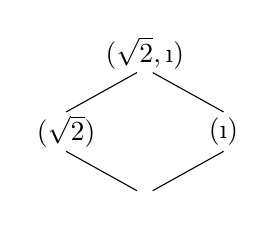
\begin{tikzpicture}
		\node at (0,0) {$\Q$};
		\node at (-1,1) {$\Q(\sqrt{2})$};
		\node at (1,1) {$\Q(\i)$};
		\node at (0,2) {$\Q(\sqrt{2},\i)$};
		\draw (-0.1,0.25) -- (-1,0.75);
		\draw (0.1,0.25) -- (1,0.75);
		\draw (-1,1.25) -- (-0.1,1.75);
		\draw (1,1.25) -- (0.1,1.75);
	\end{tikzpicture}
	\end{center}
	Frage: Gibt es noch weitere Teilkörper von $\Q(\sqrt{2},\i)$?
\end{genericdf}

\begin{df}\label{skript:13.14}
	Seien $L\supseteq K$, $f\in K[x]$, $f\neq0$ und $\Grad f\geq 1$. Man sagt, dass $f$ über $L$ in Linearfaktoren zerfällt, falls
	\[f=c\cdot(x-\alpha_1)\cdot(x-\alpha_2)\cdot\ldots\cdot(x-\alpha_n)\]
	mit $c\in K$ und $\alpha_1,\ldots,\alpha_n\in L$.\\
	Beachte: Jede Wurzel $\alpha_i$ ist algebraisch über $K$, denn $f(\alpha_i)=0$. Gilt zusätzlich, dass
	\[L=K(\alpha_1,\ldots,\alpha_n),\]
	dann nennt man $L$ einen Zerfällungskörper von $K$. Wegen $|L:K|<\infty$ (vgl. \ref{skript:13.10}) ist dann der Zerfällungskörper $L\supseteq K$ algebraisch. Gibt es $i\neq j$ mit $\alpha_i=\alpha_j$, dann nennt man $\alpha_i$ eine mehrfache Nullstelle von $f$.
\end{df}

\begin{sz}\label{skript:13.15}\
	Sei $K$ ein Körper, $f\in K[x]$ mit $\Grad f=n\geq1$. Dann existiert ein Zerfällungskörper $L\supseteq K$ von $f$ und es gilt:
	\[|L:K|\leq n!\]
\end{sz}

\begin{proof}
	Induktion nach $n$:\\
	Falls $n=1$, setze $L=K$.\\
	Sei $n>1$, $f_1\in K[x]$ irreduzibel und $f_1$ teile $f$. Nach \ref{skript:13.2} ist $K_1=K[x]/(f_1)\supseteq K$ eine Körpererweiterung mit
	\[|K_1:K|=\Grad f_1\leq n.\]
	Ferner gilt $K_1=K(\alpha_1)$ (vgl. \ref{skript:13.10} \textbf{(2)}), wobei $\alpha_1$ eine Nullstelle von $f_1$ ist. Es folgt
	\[f=(x-\alpha_1)\cdot g\text{ in }K_1[x],\]
	also ist auch $g\in K_1[x]$ und $\Grad g=n-1$. Nach Induktionsvoraussetzung existiert ein Zerfällungskörper $L\supseteq K_1$ von $g$ mit
	\[|L:K_1|\leq(n-1)!\]
	Seien $\alpha_2,\ldots,\alpha_n$ die Nullstellen von $g$. Es gilt $L=K_1(\alpha_2,\ldots,\alpha_n)$, also auch $L=K(\alpha_1,\ldots,\alpha_n)$. Somit ist $L$ Zerfällungskörper von $f$ und es gilt:
	\[|L:K|=|L:K_1|\cdot|K_1:K|\leq (n-1)!\cdot n=n!\]
\end{proof}

\begin{genericdf}{Beispiel}\label{skript:13.16}\
	$f=x^4-2\in\Q[x]$. Gesucht ist der Zerfällungskörper von $f$ über $\Q$. $\alpha=\sqrt[4]{2}$ ist eine Nullstelle von $f$. Die Linearfaktorzerlegung von $f$ ist
	\[f(x)=(x-\alpha)(x+\alpha)(x-\i\alpha)(x+\i\alpha).\]
	Dann ist
	\[L=\Q(\alpha,-\alpha,\i\alpha,-\i\alpha)=\Q(\alpha,\i\alpha)=\Q(\alpha,\i)\]
	ein Zerfällungskörper von $f$. Es gilt $|\Q(\alpha):\Q|=4$ (vgl. \ref{skript:13.5} \textbf{(2)}) und $\i\notin\Q(\alpha)$. Das Minimalpolynom von $\i$ über $\Q(\alpha)$ ist $\mu_\i=x^2+1$. Mit der Gradformel folgt schließlich:
	\[|L:\Q|=|L:\Q(\alpha)|\cdot|\Q(\alpha):\Q|=2\cdot4=8\]
\end{genericdf}

\begin{df}\label{skript:13.17}
	Ein Körper $K$ heißt algebraisch abgeschlossen, wenn jedes Polynom $f\in K[x]$ mit $\Grad f\geq 1$ über $K$ in Linearfaktoren zerfällt. $L\supseteq K$ heißt algebraischer Abschluss von $K$, wenn $L$ algebraisch abgeschlossen ist und $L\supseteq K$ algebraisch ist.
\end{df}

\begin{genericdf}{Bemerkung und Beispiele}\label{skript:13.18}\
	\begin{enumerate}
		\item[\textbf{(1)}]
		Aus der komplexen Analysis ist bekannt, dass $\C$ algebraisch abgeschlossen ist.
		\item[\textbf{(2)}]
		Ein algebraischer Abschluss von $\Q$ ist gegeben durch
		\[\overline{\Q}:=\{\alpha\in\C|\alpha\text{ ist algebraisch über }\Q\}.\]
		$\overline{\Q}$ ist nach Folgerung \ref{skript:13.12} ein Teilkörper von $\C$ (vgl. §12). Ist $f\in\overline{\Q}[x]$ mit $\Grad f=n\geq 1$, dann ist
		\[f=c\cdot\prod_{i=1}^n (x-\alpha_i)\]
		mit $c\in\overline{\Q}$, $\alpha_i\in\C$ für $1\leq i\leq n$, da $\C$ algebraisch abgeschlossen ist und
		\[f=\sum_{i=0}^n\tilde{\alpha}_ix^i\]
		mit $\tilde{\alpha}_i\in\overline{\Q}$. Setze $L=\Q(\tilde{\alpha}_0,\ldots,\tilde{\alpha}_n)$. Aus $\tilde{\alpha}_i\in\overline{\Q}$ folgt, dass $\tilde{\alpha}_i$ algebraisch über $\Q$ sind. Mit \ref{skript:13.10} \textbf{(3)} ist auch $L$ algebraisch über $\Q$. Es gilt $f(\alpha_i)=0$, also sind die $\alpha_i$ algebraisch über $L$ und $L(\alpha_i)$ ist algebraisch über $L$. Nach \ref{skript:13.11} ist nun $L(\alpha_i)$ algebraisch über $\Q$ und damit auch $\alpha_i$. Also folgt $\alpha_i\in\overline{\Q}$. D. h. $f$ zerfällt über $\overline{\Q}$ in Linearfaktoren, also ist $\Q$ algebraisch abgeschlossen.
		\item[\textbf{(3)}]
		Allgemein gilt: Jeder Körper $K$ hat einen algebraischen Abschluss. (Der Beweis verwendet das Lemma von Zorn, ist also nicht konstruktiv).
	\end{enumerate}
\end{genericdf}